\begin{appendices}
% \chapter{Sample Output}

% The models generated from LDA, BTM, and TTM all are two probability matrices, which denote the topic-document distribution and word-topic distribution respectively. The size of the topic-document distribution is K (number of topics) * 1 and the size of the word-topic distribution is K (number of topics) * W (number of words). The sample display of the model is as figure \ref{fig:14} shows, where K is the number of topics, n(W) is the number of words, p(z) is the probability of each topic in the document (topic-document distribution) and top words are the top 10 words in each topic with their probability (word-topic distribution). The sample model is generated by BTM, with the GoogleNews dataset as the training data and K is set to 15.

% \vskip 0.3in \par

% \begin{figure}[H]
%     \centering
%     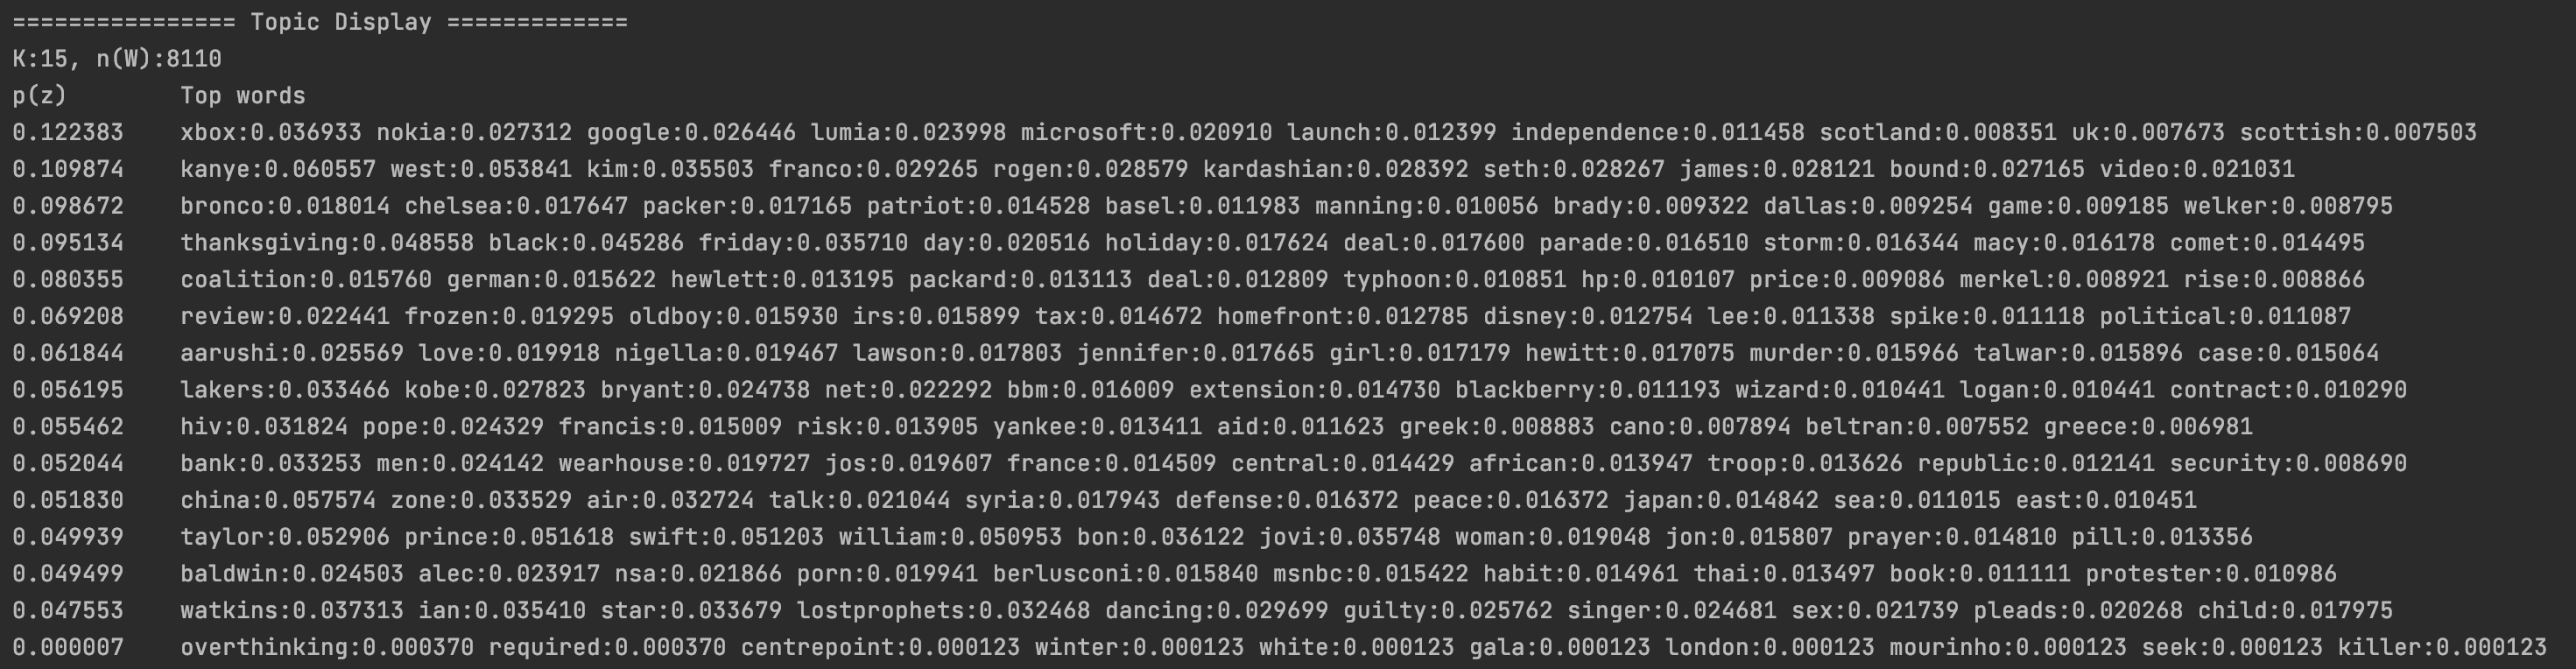
\includegraphics[scale=0.3]{images/topic_display.png}
%     \caption{Topic Display}
%     \label{fig:14}
% \end{figure}

\end{appendices}